% !TeX root = ../../../master.tex

\subsection{Result-Dashboard}
\label{ssec:ResultDashboardImplement}

Das Result-Dashboard soll die zentrale Anlaufstelle dieser Anwendung sein. 
Deshalb wird der Benutzers nach dem \emph{Login} auf diese Seite geleitet. 

Wie der Name schon sagt, sollen hier die Resultate der zuvor erstellten Umfragen einsehbar sein (vgl. Kap. \vref{ssec:UmfrageErstellen}).  
Um eine Ansprechende \ac{UI} zu generieren, soll hier auf ein \emph{Card-Design} verwendet werden. 
Über eine Button auf der Karte ist es möglich auf ein detaillierte Auswertung zu gelangen. \newline
\abb \vref{fig:SurveyResultDashboardImplement} zeigt drei erstelle Umfragen des Benutzers: 
% 
\begin{itemize}
	\item Kurzes Beispiel - WWI19SEC
	\item Projektmanagement - WWI19SEC
	\item Projektmanagement - WWI17SEC
\end{itemize}
% 
Jede Umfrage besitzt einen individuellen einzigartigen \emph{Sourveycode} wie \zb \emph{\texttt{QSDQO6EP0T}}. 
Dieser lässt sich über das Icon \faClipboard\xspace in die \emph{Zwischenablage} kopieren. 
Ferner hat der Benutzer eine Übersicht, wie viele Teilnehmer \engl{Participations} bereits an dieser Umfrage teilgenommen haben. 
Über den Button \jinline|Show Survey Results| kann der Benutzer die Ergebnisse dieser Umfrage ansehen. 

\begin{figure}[!htb]
	\centering
	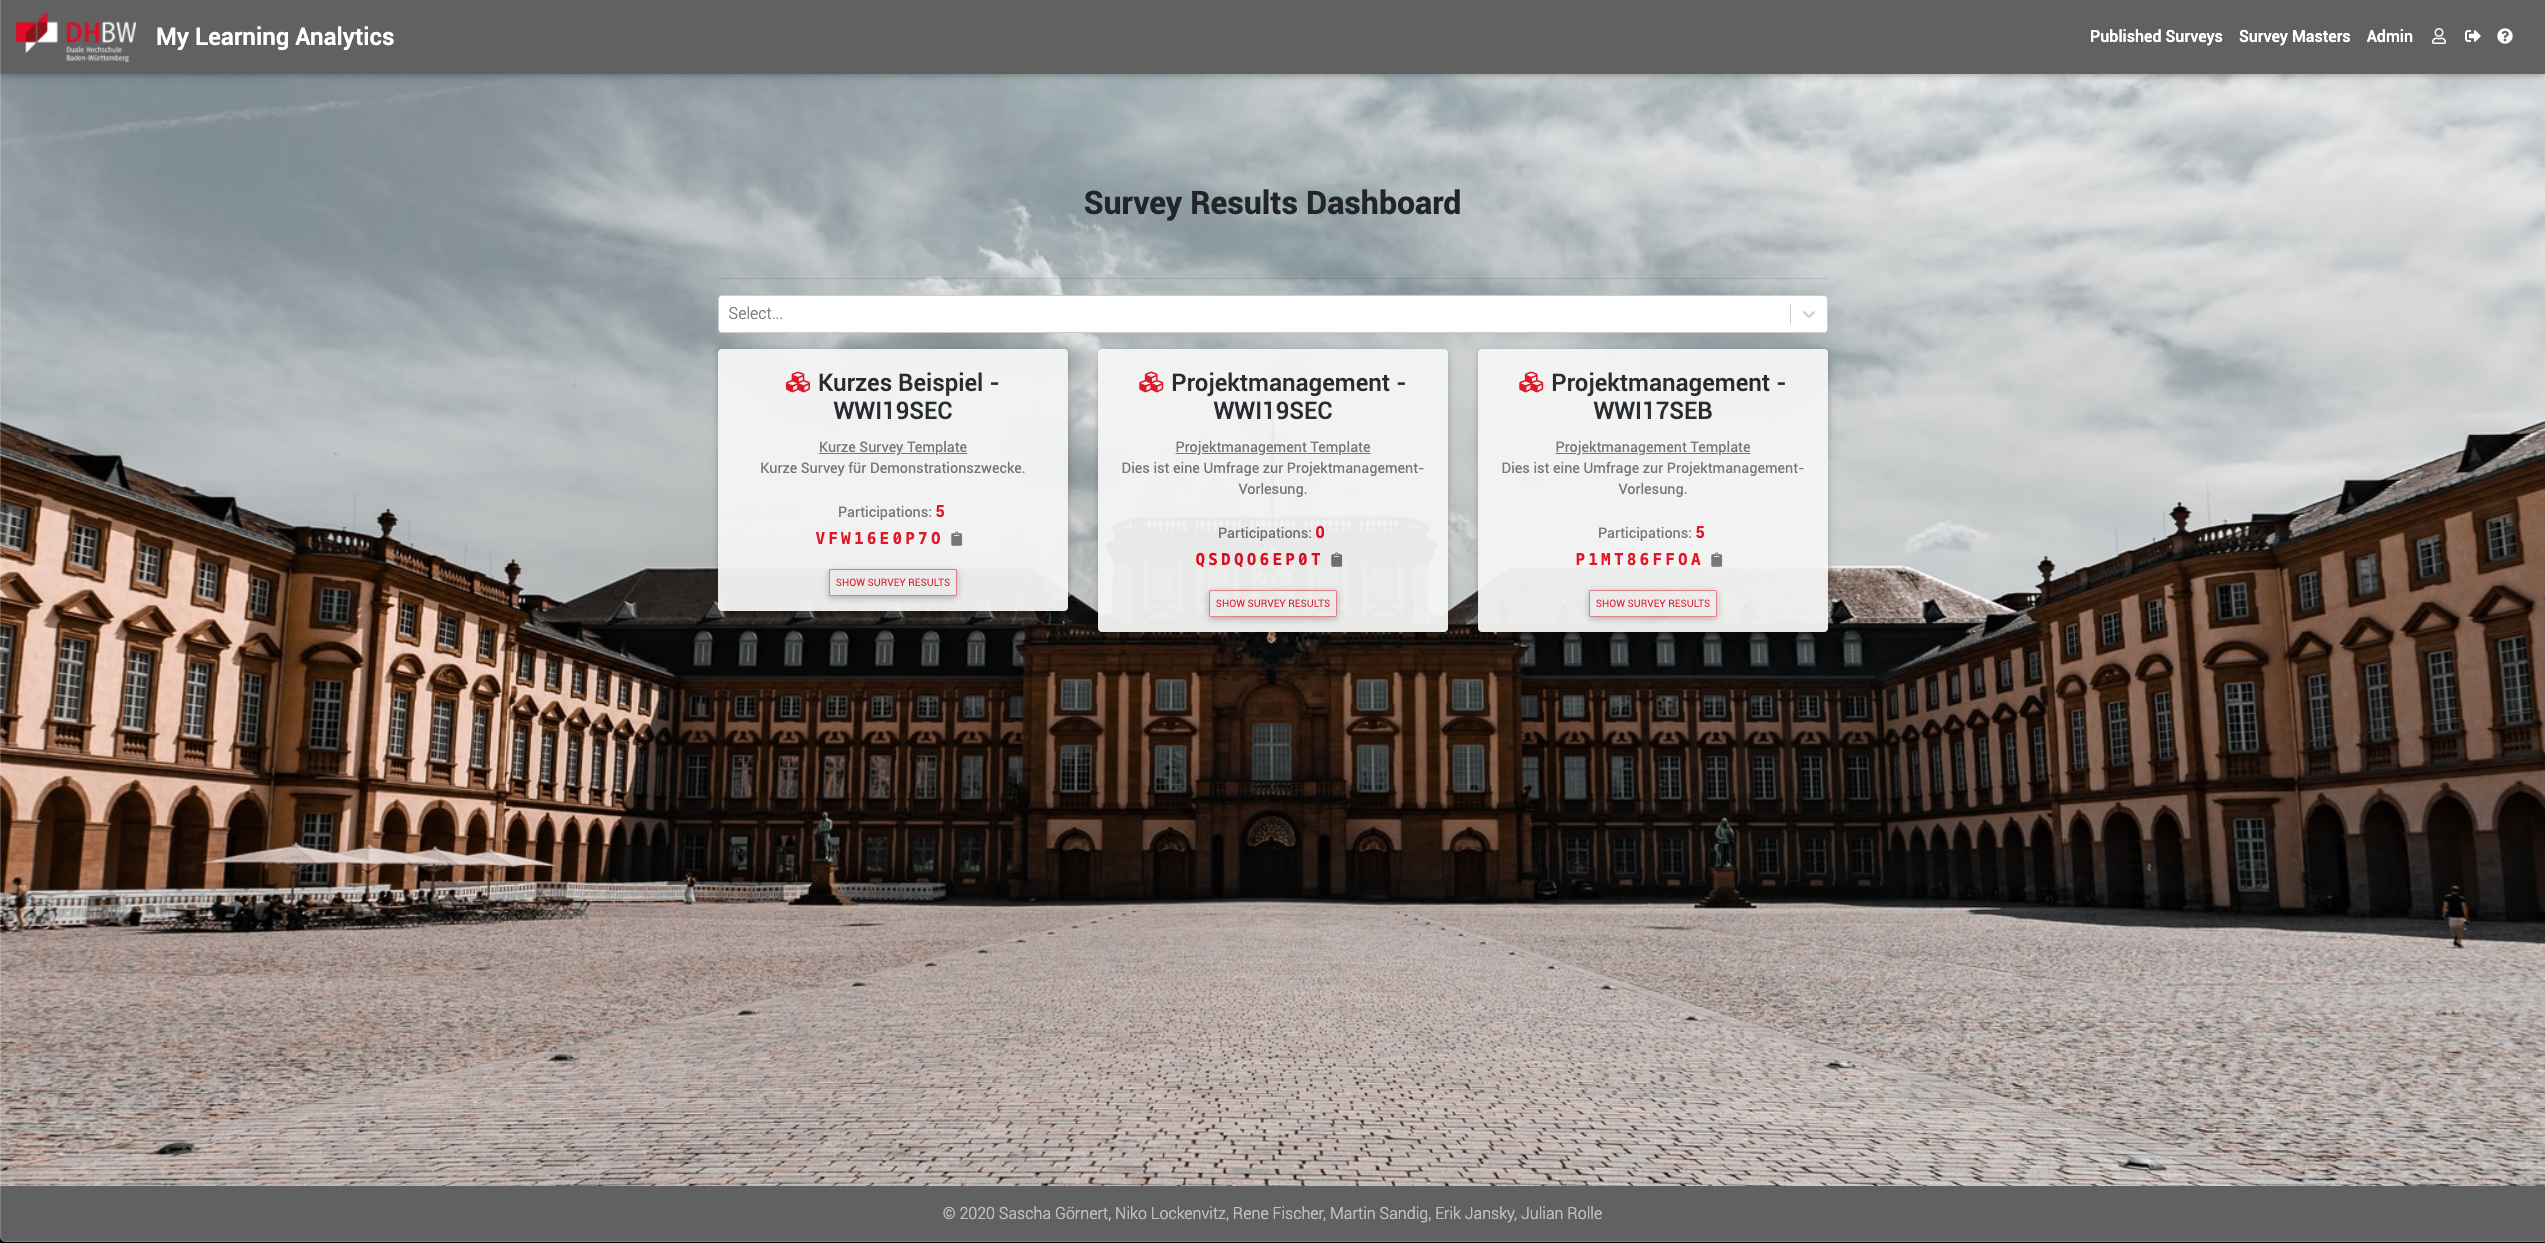
\includegraphics[width=0.95\textwidth, keepaspectratio]{img/client/SurveyResultDashboard.png}
	\captionsetup{justification=centering, format=plain}
	\caption[\acf{UI}: Result-Dashboard]{\acf{UI}: Result-Dashboard \\ \quelleScreenshot}
	\label{fig:SurveyResultDashboardImplement}
\end{figure}

\subsubsection*{Detaillierte Auswertung}
Hat der Benutzer die detaillierte Auswertung ausgwählt, soll je nach Frageart ein bestimmtes Diagramm erstellen werden. 
Die Diagramme werden mit Hilfe von \emph{react-chartjs-2} generiert.\footnote{\url{https://www.npmjs.com/package/react-chartjs-2}} 

\abb \myRefGeneral{fig:SurveyResultDetailImplement} zeigt einen Ausschnitt der Auswertung der Umfrage zur Projektmanagement-Vorlesung. 
Hier wird exemplarisch eine \emph{Tortendiagramm} ausgegeben. 
Die verwendeten Farben wurden zuvor definiert. 
Der Benutzer hat die Möglichkeit über das \emph{Tortendiagramm} mit seiner Maus zu bewegen (hovern).
Hierbei erhält er den jeweiligen Wert über einen \emph{Tooltip}\footnote{Es öffnet sich ein kleines Fenster, welches Informationen zum ausgewählten Element beinhaltet.} angezeigt.

Dadurch wird Anforderung~\hyperref[Anf:A13]{A13}, die grafische Darstellung der Umfrageergebnisse, erfüllt.

\begin{figure}[!htb]
	\centering
	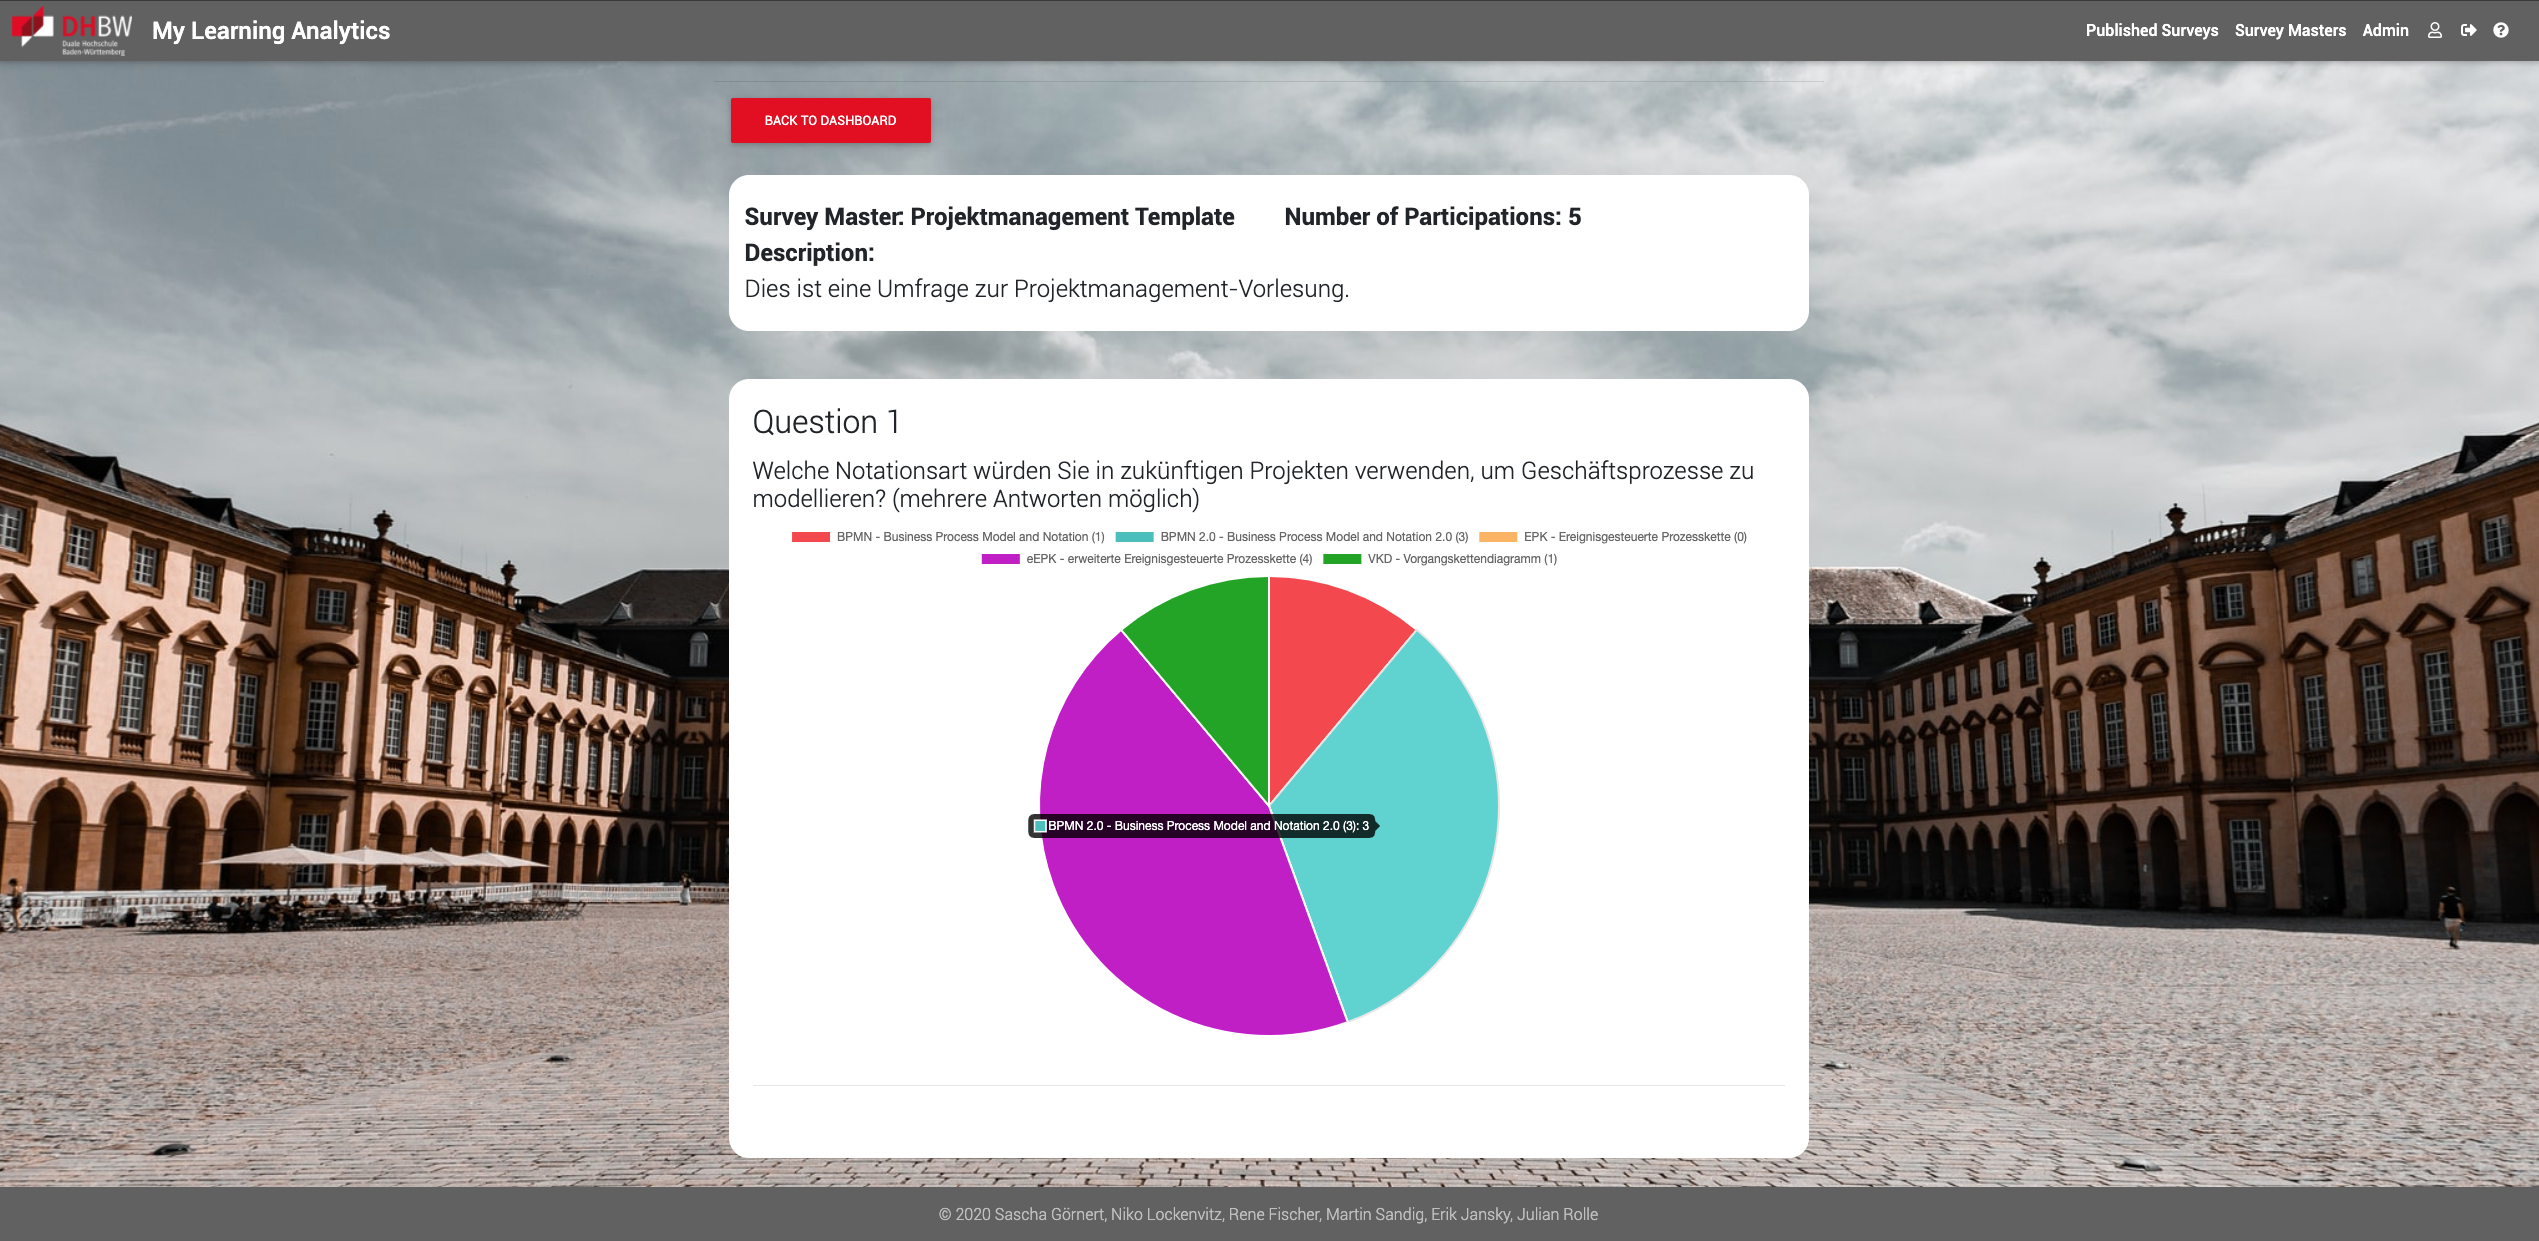
\includegraphics[width=0.95\textwidth, keepaspectratio]{img/client/SurveyResultDetail2.png}
	\captionsetup{justification=centering, format=plain}
	\caption[\acf{UI}: Auswertung der Umfrage]{\acf{UI}: Auswertung der Umfrage aus Abb. \vref{fig:SurveyResultDashboardImplement} \\ \quelleScreenshot}
	\label{fig:SurveyResultDetailImplement}
\end{figure}
